En el contexto actual de las tecnologías de la información, el \textbf{almacenamiento de datos} constituye un componente fundamental para el funcionamiento de cualquier organización. La forma en que se gestiona, estructura y accede a la información determina el rendimiento, la escalabilidad y la eficiencia de los sistemas informáticos. Dentro de las principales arquitecturas de almacenamiento disponibles hoy en día se destacan \textbf{tres} modelos fundamentales: \textbf{DAS} (Direct Attached Storage), \textbf{NAS} (Network Attached Storage) y \textbf{SAN} (Storage Area Network). Cada uno de estos modelos presenta características distintivas que los hacen adecuados para diferentes escenarios y necesidades organizacionales.

\subsubsection{Diferencias fundamentales entre acceso a bloques (SAN/FC) y acceso a archivos (NAS)}

El acceso a bloques es el modelo más cercano al hardware físico. En este modelo, los datos se dividen en unidades de tamaño fijo llamadas bloques, cada uno con un identificador único. El dispositivo de almacenamiento no tiene conocimiento sobre el contenido de los datos que almacena: no sabe si los bloques contienen partes de una base de datos, fragmentos de un archivo de video o secciones de un sistema operativo. Simplemente recibe comandos para escribir o leer bloques específicos.

Una característica fundamental es que no existe un sistema de archivos implementado por el dispositivo de almacenamiento. El dispositivo simplemente proporciona espacio de bloques crudos sin ninguna estructura organizativa. El sistema operativo del servidor que se conecta a la SAN es responsable de crear y gestionar su propio sistema de archivos sobre los bloques proporcionados, decidiendo cómo organizar los datos, qué archivos crear y cómo estructurar directorios.

El acceso a archivos representa un nivel de abstracción significativamente más alto. En este modelo, los datos se organizan en una estructura jerárquica de archivos y directorios que es gestionada por el dispositivo de almacenamiento mismo. El dispositivo no solo guarda los datos, sino que también mantiene toda la información sobre cómo están organizados, qué nombres tienen, en qué directorios se encuentran y qué metadatos están asociados.

\subsubsection{Almacenamiento Directamente Adjunto (DAS)}

El \textbf{DAS (Direct Attached Storage o Almacenamiento Directamente Adjunto)} representa el modelo de almacenamiento más sencillo y tradicional. En esta arquitectura, los dispositivos de almacenamiento están conectados directamente a un servidor o computadora cliente a través de interfaces como SATA, SAS o USB. El almacenamiento DAS no pasa por ninguna red; es decir, el disco duro o arreglo de discos está físicamente conectado al servidor que lo utiliza.

La escalabilidad del DAS es limitada, ya que está restringida por la cantidad de puertos de conexión disponibles en el servidor y por el espacio físico en el chasis del mismo. Cuando se agota la capacidad de almacenamiento de un servidor con DAS, generalmente es necesario reemplazar el servidor completo o agregar servidores adicionales, lo que puede resultar en una arquitectura fragmentada y difícil de gestionar.

A pesar de sus limitaciones, el DAS presenta ventajas significativas en términos de costo y simplicidad. Es la opción más económica debido a que no requiere inversión en infraestructura de red adicional, switches o tarjetas de interfaz especializadas, además, su configuración es sencilla.

\subsubsection{Almacenamiento Conectado a la Red (NAS)}

El \textbf{NAS (Network Attached Storage o Almacenamiento Conectado a la Red)} es un dispositivo de almacenamiento especializado que se conecta a la red existente de una organización mediante el protocolo TCP/IP. A diferencia de la SAN, el NAS \textbf{opera a nivel de archivos}, lo que significa que cuenta con su propio sistema operativo y sistema de archivos, y proporciona acceso a los datos a través de protocolos de compartición de archivos como \textbf{CIFS/SMB para sistemas Windows o NFS para sistemas UNIX/Linux}.

El NAS funciona esencialmente como un servidor de archivos dedicado. El dispositivo NAS contiene su propio sistema operativo optimizado para la gestión de archivos y proporciona servicios de almacenamiento a múltiples clientes simultáneamente a través de la red corporativa existente. Esto significa que no requiere una infraestructura de red separada, ya que comparte la misma red utilizada por los usuarios para otras tareas.

En términos de escalabilidad, el NAS ofrece una capacidad media. Puede expandirse agregando más dispositivos NAS a la red o actualizando los discos existentes, pero está limitado por el ancho de banda de la red convencional y puede experimentar cuellos de botella cuando múltiples clientes acceden intensivamente a los datos simultáneamente.


\subsection{Qué es una SAN}

Una SAN, Storage Area Network (Red de Área de Almacenamiento), es una red de alta velocidad dedicada que conecta servidores con dispositivos de almacenamiento compartidos. Esta arquitectura permite que múltiples servidores accedan a almacenamiento centralizado como si fuera almacenamiento local directo, proporcionando una infraestructura robusta para el manejo de grandes volúmenes de datos en entornos empresariales.

La SAN se caracteriza por operar a nivel de bloques, lo que significa que divide los datos en volúmenes organizados arbitrariamente y los servidores perciben el espacio de disco de la SAN como si fuera su propio disco duro físico. Esta característica es fundamental, ya que permite que los sistemas operativos y las aplicaciones apliquen sus propios sistemas de archivos sobre los bloques de almacenamiento proporcionados por la SAN.

\begin{figure}[H]
	\centering
	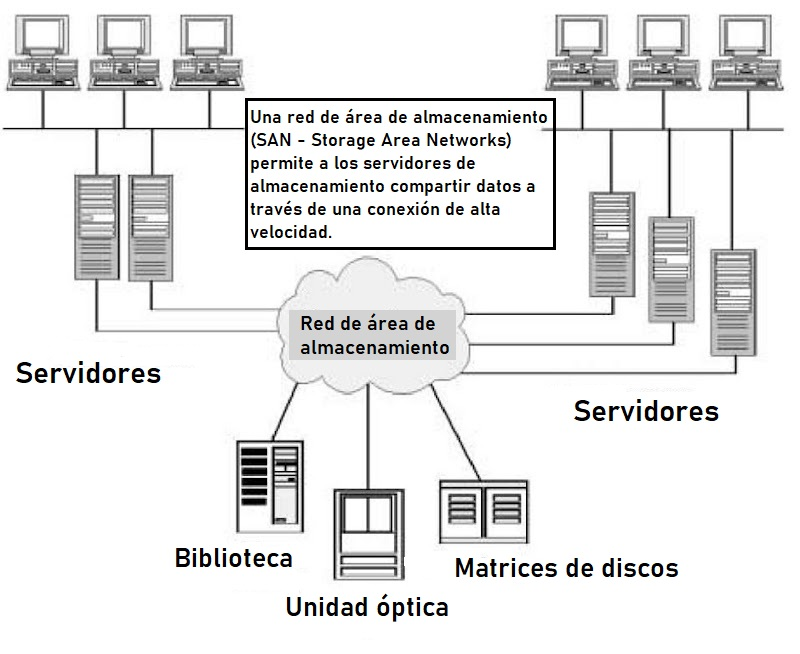
\includegraphics[width=0.5\textwidth]{img/san1.png}
	\caption{SAN}
	\label{fig:san1}
\end{figure}

\subsection{Características técnicas de una SAN}

La infraestructura de una SAN utiliza protocolos exclusivos diseñados específicamente para almacenamiento, siendo los más comunes el \textbf{Fibre Channel} y el \textbf{iSCSI}. El \textbf{Fibre Channel} es un protocolo de alta velocidad que opera a través de fibra óptica, mientras que \textbf{iSCSI} permite transportar comandos SCSI a través de redes TCP/IP convencionales, ofreciendo una alternativa más económica.

Una característica distintiva de la SAN es que cuenta con una infraestructura de red completamente independiente y separada de la red de datos convencional. Esto incluye switches, cableado y tarjetas de interfaz de red dedicados exclusivamente al tráfico de almacenamiento. La separación del tráfico de almacenamiento del tráfico de usuarios resulta en mayor rendimiento y menor latencia, ya que el tráfico intensivo de E/S de almacenamiento no compite con el tráfico regular de la red.

La capacidad de escalabilidad es prácticamente ilimitada, permitiendo agregar discos y arreglos de almacenamiento según sea necesario, llegando a manejar miles de terabytes de información. Esta característica la hace ideal para organizaciones en crecimiento que requieren flexibilidad para expandir su capacidad de almacenamiento sin interrumpir operaciones.

Desde el punto de vista del rendimiento, la SAN ofrece capacidades superiores con alto rendimiento y baja latencia, lo que la convierte en la opción preferida para aplicaciones críticas que requieren acceso rápido y constante a los datos, como bases de datos, servidores de correo y sistemas de virtualización.

\subsection{Diferencias fundamentales entre SAN, NAS y DAS}

\begin{figure}[H]
	\centering
	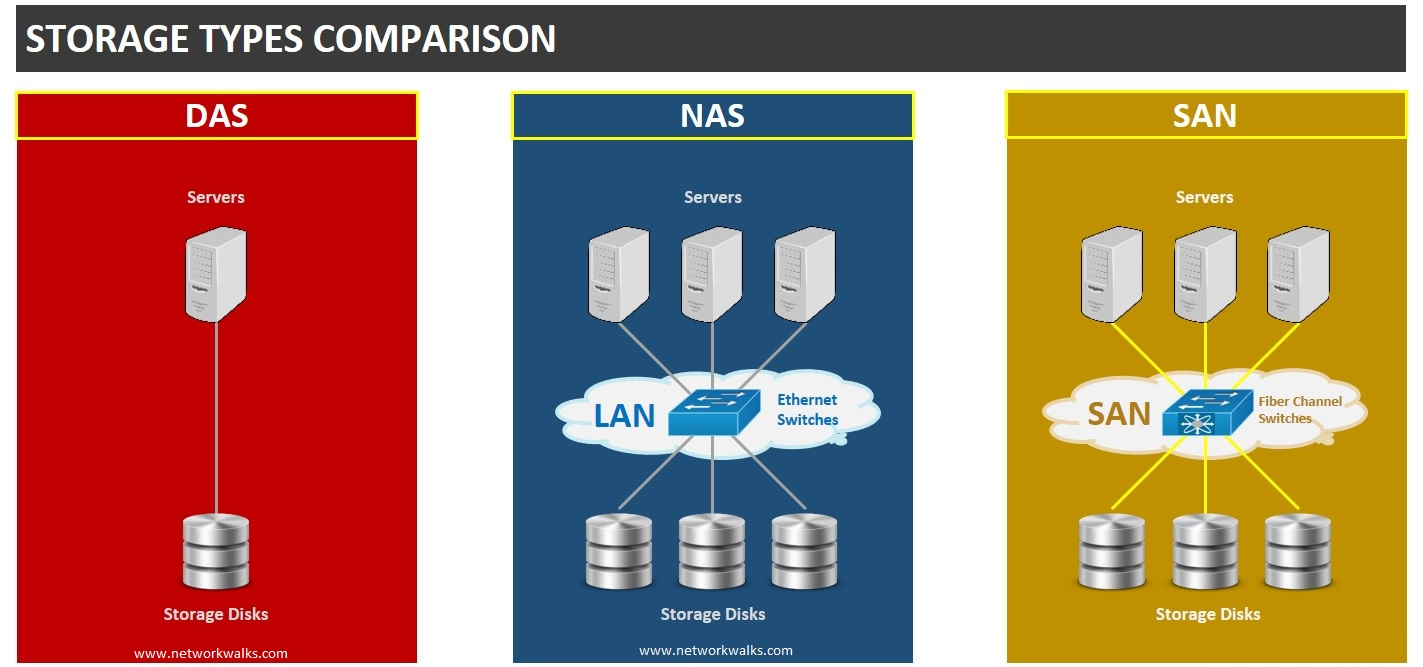
\includegraphics[width=0.8\textwidth]{img/san2.png}
	\caption{DAS - NAS - SAN}
	\label{fig:san2}
\end{figure}

\subsubsection{Nivel de acceso a los datos}

La diferencia más significativa entre estos tres modelos de almacenamiento radica en el nivel de acceso a los datos. La \textbf{SAN} opera a \textbf{nivel de bloques}, lo que significa que los datos se leen en bloques de tamaño fijo sin un sistema de archivos predefinido. Los servidores que se conectan a una SAN perciben el almacenamiento como discos locales y pueden aplicar sus propios sistemas de archivos sobre los bloques proporcionados.

El \textbf{NAS}, opera a nivel de \textbf{archivos}. El dispositivo NAS gestiona su propio sistema de archivos y proporciona acceso a los datos a través de archivos y directorios completos. Los clientes no tienen acceso directo a los bloques de datos, sino que solicitan archivos completos o partes de archivos a través de protocolos de compartir archivos.

El \textbf{DAS} también opera a \textbf{nivel de bloques}, similar a la SAN, pero con la diferencia fundamental de que el almacenamiento está físicamente conectado al servidor y no es compartible a través de una red. El sistema operativo del servidor gestiona directamente los bloques de almacenamiento sin intermediarios.

\subsubsection{Infraestructura de red}

La SAN requiere una red dedicada e independiente, con switches Fibre Channel, cableado de fibra óptica y tarjetas de interfaz especializadas. Esta separación del tráfico de almacenamiento del tráfico de usuarios resulta en mayor rendimiento y seguridad, pero también implica un costo mayor.

El NAS utiliza la red existente de la organización, aprovechando la infraestructura TCP/IP ya instalada. No requiere inversión en hardware de red adicional, lo que reduce significativamente el costo de implementación. Sin embargo, esto también significa que el tráfico de almacenamiento compite con el tráfico regular de la red, lo que puede afectar el rendimiento en situaciones de alta demanda.

El DAS no utiliza red para el acceso primario a los datos, ya que el almacenamiento está conectado directamente al servidor. Esta característica elimina los cuellos de botella de red.

\subsubsection{Capacidad de compartición y escalabilidad}

El DAS ofrece la capacidad de compartición más limitada, ya que el almacenamiento es exclusivo del servidor al que está físicamente conectado. El NAS fue diseñado específicamente para la compartición de archivos entre múltiples usuarios y sistemas. Su arquitectura permite que numerosos clientes accedan simultáneamente a los mismos archivos y directorios, gestionando los permisos de acceso de manera centralizada y eficiente.

La SAN ofrece una capacidad de compartición avanzada, permitiendo que múltiples servidores accedan simultáneamente al mismo almacenamiento físico. Sin embargo, a diferencia del NAS, la compartición en la SAN se gestiona a nivel de bloques, lo que requiere coordinación a nivel de sistema operativo o de aplicaciones para evitar conflictos de acceso a los mismos datos.

En términos de escalabilidad, la SAN es superior, ofreciendo capacidad prácticamente ilimitada para agregar discos y arreglos de almacenamiento sin necesidad de reemplazar servidores completos. El NAS ofrece escalabilidad media, limitada por el ancho de banda de la red y por la capacidad de los dispositivos NAS individuales. El DAS presenta la escalabilidad más limitada, restringida por los puertos de conexión y el espacio físico del servidor.

\subsubsection{Rendimiento y latencia}

El rendimiento es una de las principales fortalezas de la SAN. Al utilizar una red dedicada de alta velocidad con protocolos optimizados para almacenamiento, la SAN ofrece la producción más alta y la latencia más baja. Esta característica la hace ideal para aplicaciones críticas que requieren acceso rápido y constante a los datos, como bases de datos transaccionales, servidores de correo electrónico y sistemas de virtualización.

El DAS puede ofrecer rendimiento alto en escenarios de uso único, ya que no introduce los cuellos de botella de red. Sin embargo, esta ventaja desaparece cuando se necesita compartir el almacenamiento entre múltiples servidores.

El NAS ofrece rendimiento medio, con latencias mayores comparadas con la SAN debido al uso de la red convencional y a los protocolos de nivel de archivo. El rendimiento puede degradarse significativamente cuando múltiples clientes acceden intensivamente a los datos simultáneamente, especialmente si la red está congestionada.

%%

\subsection{Arquitectura general de una SAN}

La arquitectura de una SAN se compone de \text{tres capas} fundamentales que trabajan de manera integrada: la capa de host, la capa de fabric (estructura) y la capa de almacenamiento. Esta estructura en capas permite una separación clara de funciones, facilitando la gestión, la escalabilidad y la resolución de problemas en la red de almacenamiento. 

\begin{figure}[H]
	\centering
	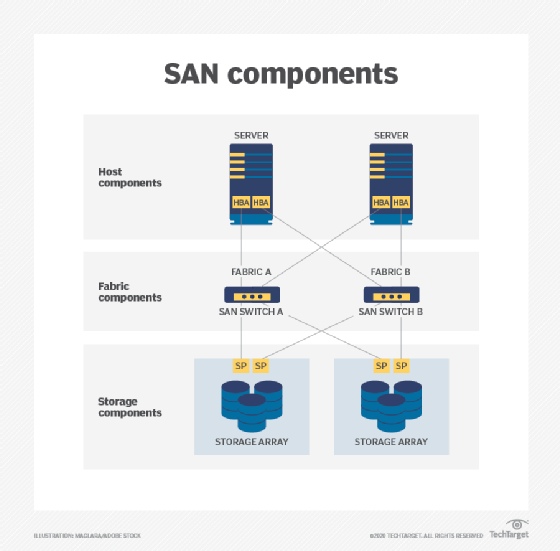
\includegraphics[width=0.7\textwidth]{img/san3.png}
	\caption{Arquitectura de una SAN}
	\label{fig:san3}
\end{figure}

\subsubsection{Capa de Host}

La capa de host constituye el primer nivel de la arquitectura SAN y está formada por los servidores que necesitan acceder al almacenamiento remoto. Estos servidores son las máquinas que ejecutan aplicaciones críticas como bases de datos, sistemas de correo electrónico, plataformas de virtualización y otros servicios empresariales que requieren acceso rápido y confiable a grandes volúmenes de datos.

El componente más importante de la capa de host es el \text{HBA (Host Bus Adapter o Adaptador de Bus de Host)}, que es una tarjeta de interfaz especializada de alta velocidad. Se trata de un hardware específicamente diseñado para conectarse a redes de almacenamiento, con características y capacidades optimizadas para el tráfico de E/S (entrada/salida) de almacenamiento.

El HBA actúa como un puente fundamental entre el servidor y la red de almacenamiento. Su función principal es traducir las solicitudes de lectura y escritura del sistema operativo del servidor al protocolo de la SAN, ya sea Fibre Channel, iSCSI u otro protocolo utilizado. Esta traducción es transparente para el sistema operativo, lo que permite que este vea el almacenamiento remoto de la SAN exactamente como si fuera un disco duro local conectado físicamente al servidor.

Los HBAs modernos incluyen capacidades de procesamiento propia, lo que descarga del procesador principal del servidor las tareas relacionadas con el almacenamiento, mejorando así el rendimiento general del sistema. Además, muchos HBAs cuentan con funciones de redundancia y failover automático, permitiendo que el servidor mantenga la conectividad con el almacenamiento incluso si falla un componente de la red.

\subsubsection{Capa de Fabric (Estructura)}
La capa de fabric, también conocida como capa de estructura, constituye el corazón de la SAN y es responsable de interconectar los servidores de la capa de host con los dispositivos de almacenamiento de la capa de almacenamiento. Esta capa es la que realmente transforma la colección de dispositivos en una red funcional y capaz de enrutar el tráfico de almacenamiento de manera eficiente y confiable.

El componente principal de esta capa son los switches SAN, que son dispositivos de interconexión especializados diseñados específicamente para manejar tráfico de almacenamiento. Estos switches no son switches de red convencionales, aunque pueden parecerse físicamente. Los switches SAN están optimizados para manejar el tráfico de E/S de almacenamiento, suele ser más intensivo en operaciones de pequeño tamaño, requiere latencias extremadamente bajas y es muy sensible a la pérdida de paquetes.

En una SAN basada en Fibre Channel, los switches FC son dispositivos especializados que utilizan el protocolo Fibre Channel para enrutar tramas entre los dispositivos conectados. Estos switches operan en un nivel similar al de los switches Ethernet en una red convencional, pero con protocolos y mecanismos específicos para almacenamiento. Los switches modernos soportan velocidades de 8 Gbps, 16 Gbps, 32 Gbps e incluso 128 Gbps por puerto, proporcionando el ancho de banda necesario para aplicaciones exigentes.

La redundancia es un aspecto crítico en la capa de fabric. En entornos empresariales críticos, es común implementar múltiples switches SAN formando una fabric redundante. Esto significa que cada servidor se conecta a dos o más switches diferentes, y cada dispositivo de almacenamiento también se conecta a múltiples switches. De esta manera, si un switch falla, el tráfico puede ser redirigido a través de los switches restantes, manteniendo la conectividad entre servidores y almacenamiento.

Los switches SAN incluyen funciones avanzadas como Zoning, que permite dividir la fabric en grupos lógicos de dispositivos que pueden comunicarse entre sí. El Zoning es similar a las VLANs en redes Ethernet y sirve para controlar qué servidores pueden acceder a qué dispositivos de almacenamiento, proporcionando seguridad y organización lógica.

Además de los switches, la capa de fabric puede incluir otros dispositivos como extenders (para conectar fabrics en diferentes ubicaciones geográficas), routers SAN (para conectar diferentes tipos de redes de almacenamiento) y gateways (para convertir entre diferentes protocolos). Estos dispositivos permiten extender la SAN más allá de un solo centro de datos y conectar diferentes tecnologías de almacenamiento.

\subsubsection{Capa de Almacenamiento}
La capa de almacenamiento contiene los dispositivos físicos donde se guardan realmente los datos. Esta capa es la que proporciona la capacidad de almacenamiento bruto que será compartida entre todos los servidores de la capa de host a través de la capa de fabric.

El componente principal de esta capa son los arrays de almacenamiento, también conocidos como controladores de almacenamiento, cabinas de discos o sistemas de almacenamiento. Un array de almacenamiento no es simplemente un conjunto de discos duros conectados entre sí. Se trata de una unidad inteligente que contiene múltiples discos, controladores especializados, memoria caché, y firmware diseñado para gestionar el almacenamiento de manera avanzada.

Los discos utilizados pueden ser discos duros mecánicos tradicionales (HDD), unidades de estado sólido (SSD), o una combinación de ambos en sistemas híbridos. La tendencia actual es hacia el uso creciente de SSD, que ofrecen velocidades de acceso mucho mayores que los discos mecánicos, aunque a un costo por gigabyte más elevado.

Una característica fundamental de los arrays de almacenamiento es la implementación de RAID (Redundant Array of Independent Disks). Es una tecnología que combina múltiples discos físicos en uno o más grupos lógicos, proporcionando redundancia de datos y mejorando el rendimiento. Existen diferentes niveles de RAID, como RAID 0, RAID 1, RAID 5, RAID 6, RAID 10, cada uno con diferentes características de rendimiento, capacidad efectiva y nivel de protección contra fallos. El array de almacenamiento gestiona automáticamente la distribución de datos y paridad entre los discos, transparentemente para los servidores que acceden al almacenamiento.

El array de almacenamiento presenta volúmenes lógicos de almacenamiento a los servidores, conocidos como LUNs (Logical Unit Numbers). Una LUN es un bloque de almacenamiento lógico que el servidor percibe como un disco duro completo. El administrador de almacenamiento puede crear múltiples LUNs a partir del mismo array, asignando diferentes capacidades a cada una según las necesidades de cada servidor o aplicación.

Los arrays modernos incluyen funciones avanzadas como thin provisioning (provisión delgada), que permite asignar más capacidad lógica que la física disponible, confiando en que no todo el espacio será utilizado realmente. También incluyen funciones de snapshot (instantáneas), que permiten crear copias instantáneas de LUNs para backup o pruebas, y funciones de replicación, que permiten copiar datos a arrays en ubicaciones remotas para recuperación ante desastres.

\subsection{Tipos de SAN}

Existen diferentes tipos de SAN definidos principalmente por el protocolo de comunicación que utilizan para transportar los comandos de almacenamiento. Cada tipo tiene características específicas en términos de rendimiento, costo, complejidad y casos de uso apropiados. Los tres tipos principales son \textbf{FC-SAN, iSCSI-SAN y FCoE-SAN.}

\subsubsection{FC-SAN (Fibre Channel SAN)}

La FC-SAN es el tipo de SAN más tradicional y ampliamente utilizado en entornos de alto nivel. Utiliza el protocolo Fibre Channel como mecanismo de transporte para los comandos de almacenamiento. Fibre Channel es un protocolo de alto rendimiento diseñado específicamente para almacenamiento, con características optimizadas para bajo latencia y alta fiabilidad.

La infraestructura de una FC-SAN requiere hardware especializado que incluye HBAs de Fibre Channel instalados en los servidores, switches de Fibre Channel dedicados y cableado de fibra óptica. Este hardware es significativamente más costoso que el hardware de red Ethernet convencional.

Las FC-SAN ofrecen el rendimiento más alto entre todos los tipos de SAN, con latencias extremadamente bajas y ancho de banda elevado. Este rendimiento superior las hace ideal para aplicaciones críticas que requieren acceso rápido y constante a los datos.

La fiabilidad de Fibre Channel es excepcional, con mecanismos de transporte que garantizan la entrega de paquetes y minimizan la pérdida de datos. El protocolo incluye mecanismos de flujo y control que previenen la congestión y aseguran que el tráfico de almacenamiento no sea afectado por picos de demanda.

Sin embargo, la FC-SAN presenta desventajas significativas. El costo es la principal desventaja, ya que el hardware especializado de Fibre Channel es mucho más costoso que el hardware Ethernet equivalente. Además, la implementación y gestión de una FC-SAN es más compleja, requiriendo personal con conocimientos especializados en tecnologías de Fibre Channel. La curva de aprendizaje es pronunciada y los administradores deben estar familiarizados con conceptos específicos de FC como Zoning, WWN (World Wide Name), LUN masking y otras terminologías y prácticas específicas.

\subsubsection{iSCSI-SAN (Internet Small Computer Systems Interface SAN)}

La iSCSI-SAN es un tipo de SAN que utiliza el protocolo iSCSI para transportar comandos SCSI a través de redes TCP/IP convencionales. iSCSI encapsula los comandos de almacenamiento SCSI dentro de paquetes TCP/IP, permitiendo que el tráfico de almacenamiento viaje a través de infraestructura de red Ethernet estándar. 

La arquitectura de una iSCSI-SAN puede utilizar hardware de red Ethernet convencional, que es más económico que el hardware de Fibre Channel. Los servidores pueden utilizar adaptadores de red Ethernet estándar o, para mejor rendimiento, adaptadores especializados llamados iSCSI HBAs o TOE (TCP Offload Engine) que descargan del procesador principal las tareas relacionadas con el protocolo TCP/IP.

En términos de rendimiento, las iSCSI-SAN modernas con redes de 10 Gbps o mayores pueden ofrecer rendimiento comparable a FC-SAN en muchos escenarios. Las latencias son ligeramente mayores que en FC debido al procesamiento adicional de TCP/IP.

La iSCSI-SAN es altamente escalable y flexible. Se puede implementar en infraestructura de red existente, aprovechando switches y cableado Ethernet ya instalados. También es fácil de expandir agregando más puertos Ethernet o actualizando a switches de mayor velocidad.

En redes congestionadas o mal configuradas, el tráfico de almacenamiento puede competir con el tráfico de datos convencional, resultando en latencias variables y rendimiento inconsistente. Para mitigar esto, es recomendable implementar VLANs dedicadas para almacenamiento o utilizar QoS (Quality of Service) para priorizar el tráfico de iSCSI.

\subsubsection{FCoE-SAN (Fibre Channel over Ethernet SAN)}

La FCoE-SAN representa un enfoque híbrido que combina las ventajas de Fibre Channel y Ethernet. FCoE encapsula tramas de Fibre Channel dentro de paquetes Ethernet, permitiendo que el tráfico de Fibre Channel viaje a través de infraestructura de red Ethernet. Esto significa que se puede utilizar el protocolo y las aplicaciones de gestión de Fibre Channel sobre hardware Ethernet más económico.

La arquitectura de FCoE requiere adaptadores de red especializados llamados Converged Network Adapters (CNA) que pueden manejar tanto tráfico de red convencional como tráfico de Fibre Channel sobre Ethernet. Estos CNAs son más costosos que las tarjetas de red Ethernet convencionales pero más económicos que los HBAs de Fibre Channel puros. Los switches requieren ser switches Ethernet que soporten FCoE, a menudo llamados FCoE-enabled switches o DCB (Data Center Bridging) switches.

El objetivo principal de FCoE es consolidar las redes de almacenamiento y redes de datos en una sola infraestructura física. En lugar de mantener dos redes separadas (una LAN Ethernet y una SAN FC), FCoE permite que ambas compitan la misma infraestructura de cableado y switches. Esta consolidación reduce significativamente la cantidad de cables, puertos en servidores y dispositivos de red, simplificando el centro de datos y reduciendo costos de capital y operación.

En términos de rendimiento, FCoE puede ofrecer rendimiento similar a Fibre Channel nativo, ya que utiliza el mismo protocolo de capas superiores. Sin embargo, requiere una infraestructura Ethernet que soporte Data Center Bridging (DCB), un conjunto de extensiones a Ethernet que proporciona entrega sin pérdida de paquetes y priorización de tráfico. Sin DCB, FCoE no puede funcionar correctamente porque la pérdida de paquetes Ethernet no es aceptable para el tráfico de Fibre Channel.

FCoE presenta ventajas interesantes pero también desafíos significativos. La consolidación de redes reduce el costo y la complejidad física del centro de datos. Sin embargo, la tecnología es más compleja de implementar y gestionar, requiriendo conocimientos tanto de Fibre Channel como de Ethernet avanzado. Además, FCoE ha encontrado adopción limitada en el mercado, ya que muchas organizaciones han optado directamente por iSCSI para redes basadas en Ethernet o han permanecido con FC tradicional para máximo rendimiento.